%-=-=-=-=-=-=-=-=-=-=-=-=-=-=-=-=-=-=-=-=-=-=-=-=
%	DOCUMENT CLASS "TEMPLATE"
%-=-=-=-=-=-=-=-=-=-=-=-=-=-=-=-=-=-=-=-=-=-=-=-=

\documentclass[a4paper]{article}
\usepackage[margin=1in]{geometry}
\usepackage{ibcat5ia}
\usepackage{calc}
\usepackage{setspace}
\usepackage{tabto}
\usepackage{tikz}
\usepackage{wrapfig}
\usepackage{floatrow}
\usepackage{verbatim}
\usepackage{array}
\usepackage{amsmath}
\usepackage{multirow}
\usepackage{biblatex}
\addbibresource{bibliography.bib}
\usepackage[framemethod=tikz]{mdframed}
\newcommand{\halmos}{$\square$} 
\usepackage{opencolor}
\usepackage{fancyhdr}
\usepackage[T1]{fontenc}
\usepackage{titlesec, blindtext, color}
\usepackage[export]{adjustbox}
\usepackage{setspace}
\pagestyle{fancy}
\fancyhf{}
\renewcommand{\headrulewidth}{0pt}
\renewcommand{\footrulewidth}{1pt}
\rfoot{\thepage}
\lfoot{\textbf{Candidate no.:} \textit{jbt806}}

\definecolor{gray75}{gray}{0.75}
\newcommand{\hsp}{\hspace{20pt}}
\titleformat{\section}[hang]{\LARGE\bfseries}{\thesection\hsp\textcolor{gray75}{|}\hsp}{0pt}{\bfseries}

\date{\vspace{-5ex}}
\newfloatcommand{capbtabbox}{table}[][\FBwidth]

\captionsetup[figure]{margin=1.5cm,font=small,labelfont={bf},name={Figure},labelsep=colon,textfont={it}}
\captionsetup[table]{margin=1.5cm,font=small,labelfont={bf},name={Table},labelsep=colon,textfont={it}}



\doublespacing
\begin{document}
\begin{titlepage}
\centering
{\LARGE\bfseries Exploring the Travelling Salesperson problem}

\vspace{1cm}

{\Large Maths Analysis and Approaches HL Internal assessment}

\vspace{1cm}

{\large Candidate no. : jbt806}

% \vspace{2cm}

% {\bfseries Submitted in fulfillment of the degree \ldots}

\vfill

{\itshape No. of pages: 16}
\end{titlepage}
% \maketitle
% \newpage
%-=-=-=-=-=-=-=-=-=-=-=-=-=-=-=-=-=-=-=-=-=-=-=-=
%
%	SECTION: Introduction
%
%-=-=-=-=-=-=-=-=-=-=-=-=-=-=-=-=-=-=-=-=-=-=-=-=

\section{Introduction}
One day our CAS advisor was talking to us about all the CAS projects that we can take up in the school. Each senior leading the project would come up and give a brief description about the project. Now you may ask what is so great about that. One project that stuck with me was a project where we would help the person who delivers coffee around the school learn new skills. How could that in any way be related to a maths IA? It was not so much the project that stimulated my curiosity. It was the current job of the individual: delivering coffees. I distinctly recall thinking to myself if I was in his shoes what path would I take in order to optimise my coffee delivery locations around school? This led me to explore the problem for my Maths IA. \\
To formulate the problem I utilised google maps to mark locations around my school and utilised the measuring tool to get the distance between the points.

\section{Introductory Problem}
A delivery boy wants to delivery coffees to various classrooms around the school. He wants to find a path such that he travels from the cafe to the classrooms and returns back to the cafe travelling the shortest distance expending the least amount of energy. Find this path. The locations around the school have been shown in  Figure \ref{fig:CoffeeMap}.
\begin{figure}[H]
        \centering
        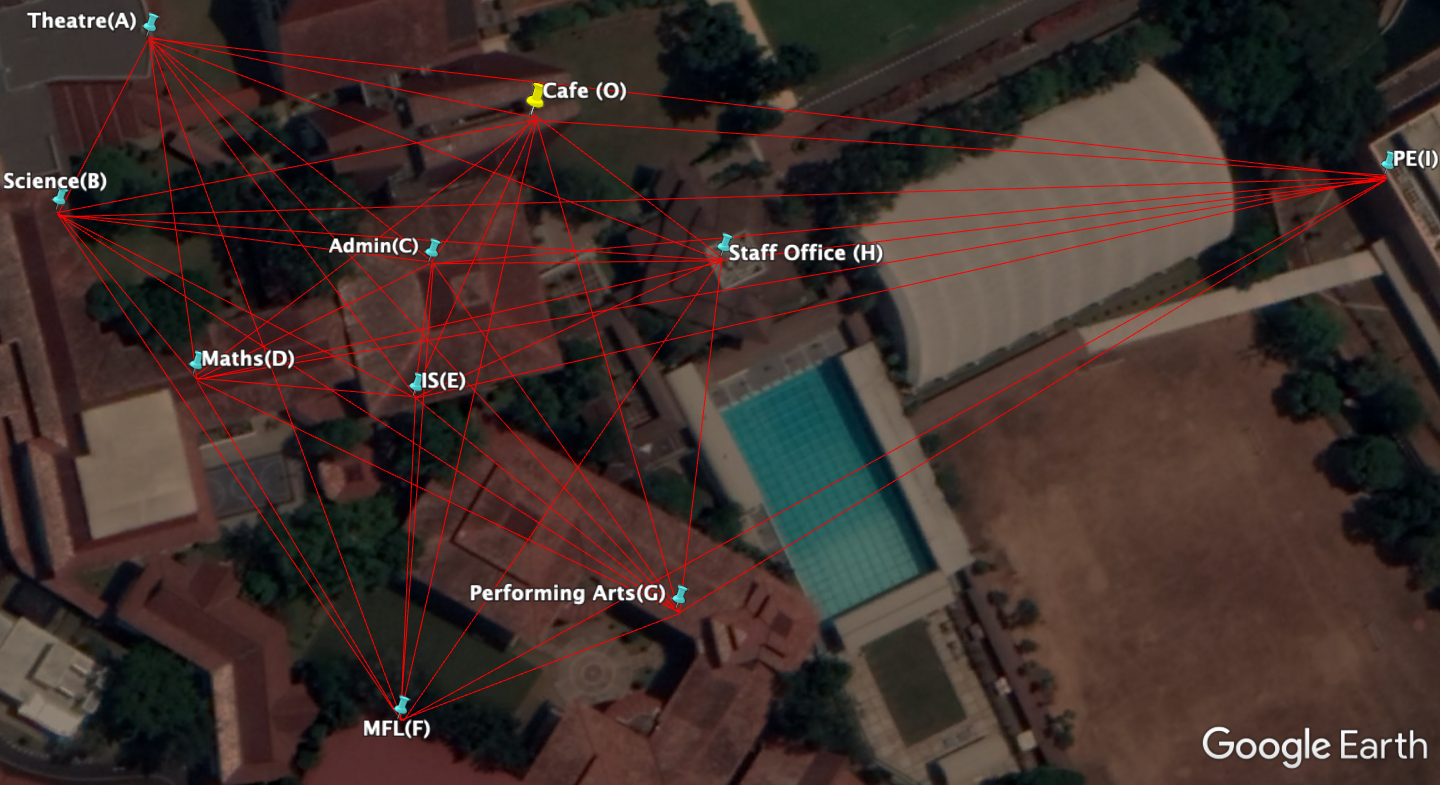
\includegraphics[width=\textwidth]{images/CoffeeMap.png}
        \caption{Coffee delivery locations on Google Maps}
        \label{fig:CoffeeMap}
\end{figure}
Table \ref{tab:CoffeeCostMatrix} shows the distance between each and every location around the school. For example the distance between point O and A is 83.
\begin{table}[H]
        \centering
        \begin{tabular}{c|cccccccccc}
        $\sim$& \textbf{O}&\textbf{A}&\textbf{B}&\textbf{C}&\textbf{D}&\textbf{E}&\textbf{F}&\textbf{G}&\textbf{H}&\textbf{I} \\ \hline
        \textbf{O}&0  &83 &102&38 &89 &63 &128&107&50 &179\\
        \textbf{A}&83 &0  &41 &75 &72 &93 &151&162&128&261\\
        \textbf{B}&102&41 &0  &78 &46 &84 &127&154&139&278\\
        \textbf{C}&38 &75 &78 &0  &55 &28 &96 &89 &61 &201\\
        \textbf{D}&89 &72 &46 &55 &0  &46 &83 &112&112&252\\
        \textbf{E}&63 &93 &84 &28 &46 &0  &67 &71 &71 &209\\
        \textbf{F}&128&151&127&96 &83 &67 &0  &63 &117&235\\
        \textbf{G}&107&162&154&89 &112&71 &63 &0  &74 &173\\
        \textbf{H}&50 &128&139&61 &112&71 &117&74 &0  &141\\
        \textbf{I}&179&261&278&201&252&209&235&173&141&0  \\
        \end{tabular}
        \caption{Distances between points for coffee delivery}
        \label{tab:CoffeeCostMatrix}
    \end{table}

%-=-=-=-=-=-=-=-=-=-=-=-=-=-=-=-=-=-=-=-=-=-=-=-=
%
%	SECTION: Travelling Salesperson Problem
%
%-=-=-=-=-=-=-=-=-=-=-=-=-=-=-=-=-=-=-=-=-=-=-=-=

\section{Travelling salesperson problem(TSP)}
The \textbf{Travelling Salesperson Problem(TSP)} is one of the widely studied combinatorial optimisation problems in the world. It was first mathematically explored by the Irish mathematician Sir William Rowam Hamilton along with British mathematician Thomas Penyngton Kirkman in the 1800's. However, the general form of the problem is believed to have been studied by Austrian mathematician Karl Menger in the 1930's.



\subsection{Definition}
Table \ref{tab:setNotation} defines the set notation that are essential to the mathematical formulation of the TSP. These notations will be used throughout this internal assessment.
\begin{table}[H]
\begin{tabular}{|c|l|}
\hline
Notation & \multicolumn{1}{c|}{Definition}  \\ \hline
$\{ \}$    & A Set of objects. E.g. $A=\{1, 2, 3, 4\}$ or $B=\{\textnormal{apple, orange, banana}\}$              \\ \hline
$\in$    & \begin{tabular}[c]{@{}l@{}}Is a member of.  E.g. $1\in A$, 1 is a member of set $A$ as defined above.\end{tabular}   \\ \hline
$\notin$ & \begin{tabular}[c]{@{}l@{}}Is not a member of. E.g. $\textnormal{grape} \notin B$, grape is not a member of set $B$ \\as evident from above.\end{tabular}            \\ \hline
\end{tabular}
\caption{Notations}
\label{tab:setNotation}
\end{table}
The TSP owes its name to the problem of determining the optimal journey of a salesperson who needs to visit $n$ cities and return back to the starting point after his journey is over. The empirical form of the problem can be defined as follows with the help of the variables shown in Table \ref{tab:tspVariables}. 
\begin{displayquote}
    \begin{table}[H]
    \begin{tabular}{|l|l|}
    \hline
    \multicolumn{1}{|c|}{Variable} & \multicolumn{1}{c|}{Definition}\\ \hline
    $\mathcal{N}$  & Set of cities salesman needs to travel   \\ \hline
    $m,n$  & Any two city pairs which are in set $\mathcal{N}$\\ \hline
    $\overline{mn}$ & The path between any two cities $m,n$.  \\ \hline
    $\mathcal{E}$  & Set of paths for for every city pair in $\mathcal{N}$                                             \\ \hline
    $c_{\overline{mn}}$ & \begin{tabular}[c]{@{}l@{}}Cost to go between a city pair.\\ Cost is referred to as the value that is being optimised.\\ This could be the time to travel between the two cities \\ or the distance between two cities. E.g. In our \\ introductory problem cost would be defined as the distance \\ between two coffee delivery locations as we are trying to \\ optimise the distance.\end{tabular}                                    \\ \hline
    $\mathcal{C}$ & \begin{tabular}[c]{@{}l@{}}Set of the costs to travel between any city pair $m,n$ for all\\ the cities in $\mathcal{N}$\end{tabular}                                \\ \hline
    \end{tabular}
    \caption{Variables}
    \label{tab:tspVariables}
    \end{table}
    \begin{center}
        For a set of finite points $\mathcal{N}$ the cost to travel between the points $m,n \in \mathcal{N}$ is defined as $c_{\overline{mn}} \in \mathcal{C}$ for all $ {\overline{mn}}  \in \mathcal{E} $. A tour is defined as a path which travels through every point in $\mathcal{N}$ exactly once. Which tour requires the least cost?\citep{3}\\
        \label{def:tsp}
    \end{center}
\end{displayquote}
The introductory problem defined earlier on is an example of a TSP. Thus we can use mathematical modelling that is used to solve TSP to find a solution for the introductory problem.
\subsection{Classifications}
In general, TSP can be classified as following:
\paragraph*{Symmetric Travelling Salesperson Problem (sTSP)}: In a sTSP the cost $c_{\overline{mn}} \in \mathcal{C}$ to travel between any two cities $(m,n) \in \mathcal{N}$ is the same both ways.
\begin{center}
    $c_{\overline{mn}}=c_{\overline{nm}}$
\end{center}
The introductory problem is a representation of an sTSP. This is evident because the cost which is the distance between any two coffee delivery locations is the same both ways. For examples if you take a look at the distance to travel from $A\rightarrow B$ is $41$ and the distance to travel from $B \rightarrow A$ is also 41.
\begin{center}
    $c_{\overline{AB}} = c_{\overline{BA}} = 41$
\end{center}
Same goes for all the other coffee delivery locations. Thus the introductory problem can be classified as a Symmetric  Travelling  Salesperson  Problem(sTSP).
\paragraph*{Asymmetric Travelling Salesperson Problem (aTSP)}: In an aTSP  unlike the sTSP the cost $c_{\overline{mn}} \in \mathcal{C}$ to travel between any two cities $(m,n)\in \mathcal{N}$ is not the same both ways. The Example 1 below shows an aTSP.
\begin{displayquote}
    \textbf{Example 1}\\
   Suchir, an extremely paranoid person, is planning to make a trip out to the supermarket, pharmacy, restaurant and the bookstore. He wants to make sure when he makes the trip he is travelling the least amount of distance so as to avoid exposure to people outside as he is in the midst of a pandemic. Which path would be the best for him. Find the shortest path.\\
   Table \ref{tab:suchirCostMatrix} gives the distances between all the locations he needs to visit.  In a mathematical modelling of the TSP such a table is referred to as the cost adjacency matrix.  It is a matrix that defines the cost which is the variable that is being optimised.
 
    \begin{figure}[H]
        \centering
        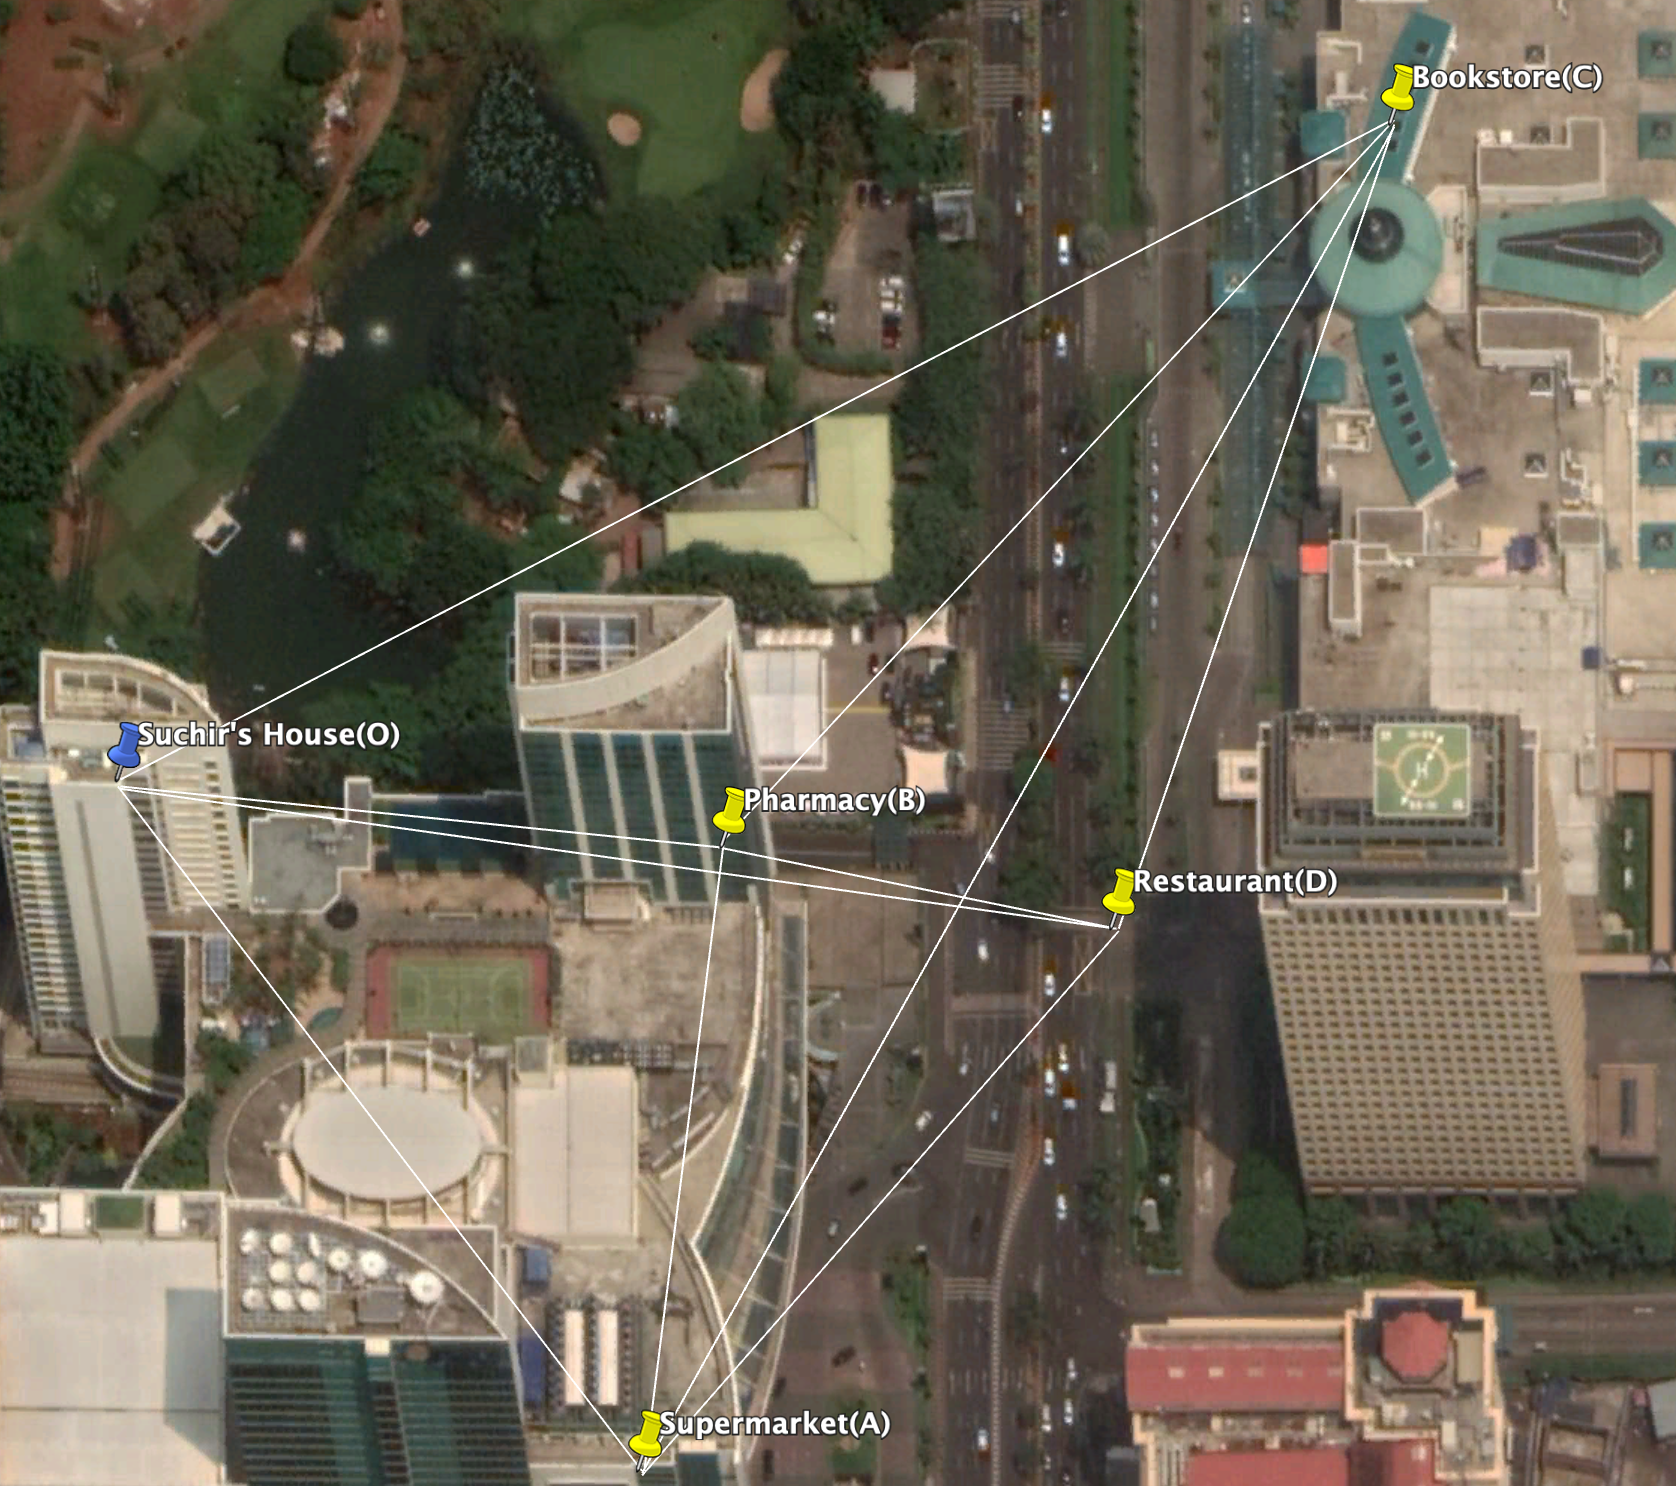
\includegraphics[width=150mm,scale=0.5]{TSP/images/suchir.png}
        \caption{Pub crawl locations on Google Maps}
        \label{fig:suchir}
    \end{figure}
    \begin{table}[H]
        \centering
        \begin{tabular}{c|ccccc}
        $\sim$ &\textbf{O}&\textbf{A}&\textbf{B}&\textbf{C}&\textbf{D}\\ \hline
        \textbf{O}& 0   & 170 & 120 & 283 & 199\\
        \textbf{A}& 147 & 0   & 124 & 304 & 143\\
        \textbf{B}& 137 & 106 & 0   & 195 & 81\\
        \textbf{C}& 276 & 302 & 182 & 0   & 167\\
        \textbf{D}& 204 & 134 & 70  & 179 & 0\\
        \end{tabular}
        \caption{Cost adjacency matrix for Suchir's trip}
        \label{tab:suchirCostMatrix}
    \end{table}
\end{displayquote}
As you can see from Table \ref{tab:suchirCostMatrix} the cost(distance) from $O\rightarrow A$ is no equal to the cost(distance) to go from $A \rightarrow A$.
\begin{center}
    $c_{OA} \neq c_{AO}$
\end{center}
\begin{figure}[H]
        \centering
        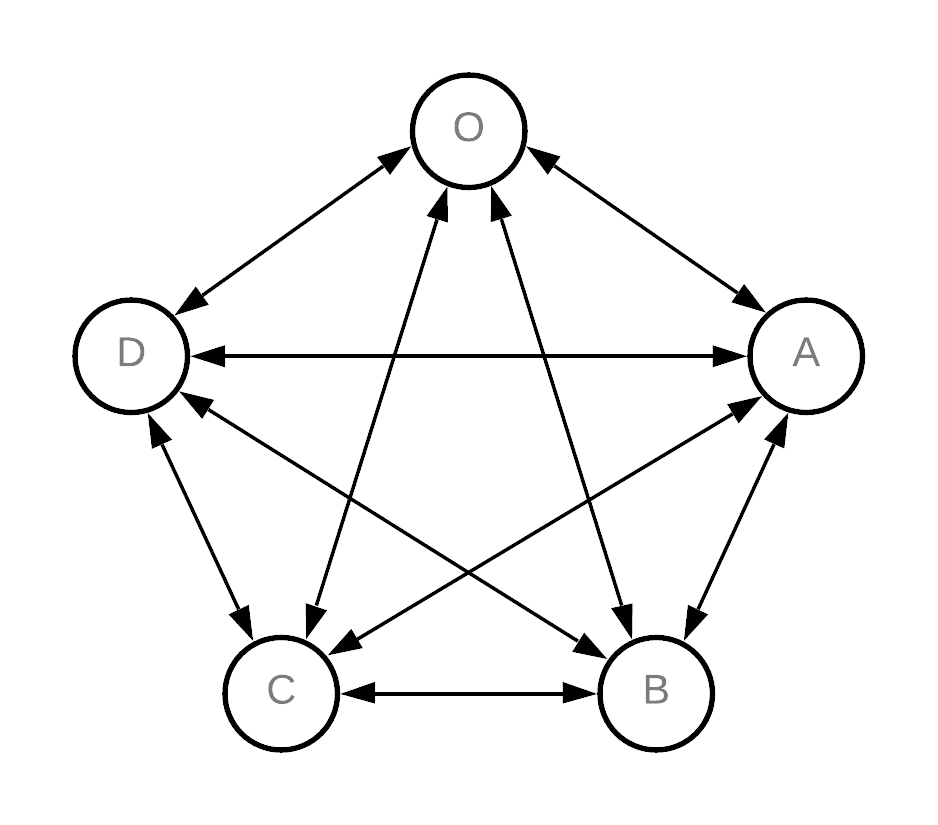
\includegraphics[width=100mm,scale=0.5]{TSP/images/suchirGraph.png}
        \caption{Directed Graph of Suchir's trip}
        \label{fig:suchirGraph}
    \end{figure}
This tells us the Example 1 is an examples of an aTSP. The graph of an aTSP needs to represented as a directed graph. Such as the one shows in Figure \ref{fig:suchirGraph}
\paragraph*{Multi Travelling Salesperson Problem (mTSP)} mTSP involves $m$ salesmen travelling and $n$ nodes and visiting those nodes exactly once in order to minimise costs.

\subsection{Mathematical Modelling}
In mathematics, TSP can be modelled using the principles of Graph Theory and integer linear programming. Let's utilise Example 1 to explore Graph Theory and model a simple TSP.
\begin{displayquote}
    \textbf{Example 2}\\
    Mark is planning to go for a pub crawl in the city of Kilkenny. He wants to visit his 3 favourite pubs in the city: O Riadas, Biddy Early's and Lenehans. However, as he is a student he has a limited amount of fuel in his car. He is trying to decide in what order should he visit the pubs to minimise the amount of fuel spent on his trip to the pubs and back. Help him plan out his pub crawl. \\
    Table \ref{tab:markCostMatrix} gives the distances between all the locations Mark needs to visit. In a mathematical modelling of the TSP such a table is referred to as the \textbf{Cost adjacency matrix}. It is a matrix that defines the cost which is the variable that is being optimised. To simplify the problem the displacement between locations is taken instead of the distance as evident in Figure \ref{fig:mark}.

    \begin{figure}[H]
        \centering
        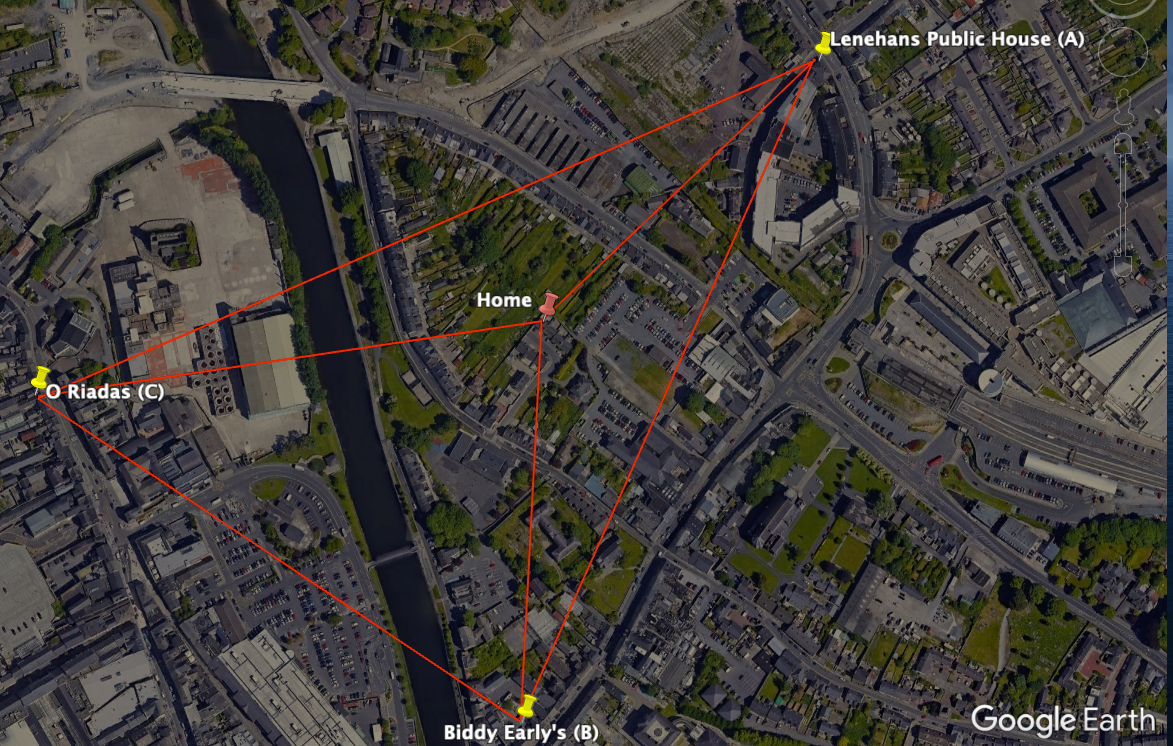
\includegraphics[width=130mm,scale=0.5]{images/PubCrawl.png}
        \caption{Pub crawl locations on Google Maps}
        \label{fig:mark}
    \end{figure}
    \begin{table}[H]
        \centering
        \begin{tabular}{c|cccc}
        $\sim$      & \textbf{O} & \textbf{A} & \textbf{B} & \textbf{C} \\ \hline
        \textbf{O}  & 0         & 294         & 307         & 394\\
        \textbf{A} & 294        & 0           & 557         & 656\\
        \textbf{B} & 307        & 557         & 0           & 448\\
        \textbf{C} & 394        & 656         & 448         & 0\\
        \end{tabular}
        \caption{Cost adjacency matrix for Mark's pub crawl
        }
        \label{tab:markCostMatrix}
    \end{table}
\end{displayquote}
\paragraph{Graph Theory} involves the exploration of graphs to study the relationship between object pairs.\citep{4} To model the TSP using Graph theory locations are defined as \textbf{nodes/vertices} and the path between $2$ locations is defined as an \textbf{edge/link}. To make it simpler to study the TSP using Graph Theory we assume that the graph is complete. This means that every node is connected to every other node by an edge. In the case where the graph is not complete a very long edge is made between the two nodes assuming that such a long edge would never appear in the optimal solution. Modelling Example 2 using graph theory would give us the below graph.
\begin{figure}[H]
    \centering
        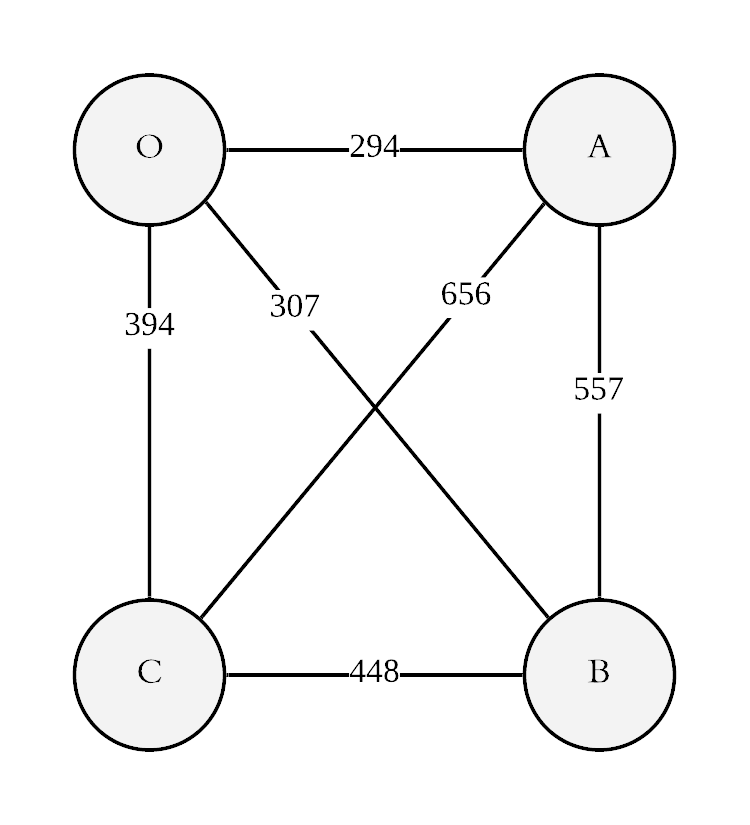
\includegraphics[width=90mm,scale=0.5]{TSP/images/PubCrawlGraph.png}
        \caption{Graph of Mark's pub crawl}
        \label{fig:markGraph}
\end{figure}
\textbf{Figure \ref{fig:markGraph}} displays a graph $\mathcal{G} = \{\mathcal{N},\mathcal{E}\}$ where $\mathcal{N} = \{O, A, B ,C \}$ defines the nodes of the graph and $\mathcal{E} = \{\overline{OA},\overline{OB}...\overline{AC},\overline{BC}\}$ defines the edges. In addition to this $\mathcal{C}=\{c_{\overline{OA}},c_{\overline{OB}}...c_{\overline{AC}}, c_{\overline{BC}} \}$ for all elements in $\mathcal{E}$. A tour here is defined as the path/circuit in $\mathcal{G}$ where the path meets every point on the graph. This circuit where the path visits each node exactly only once is known as a Hamiltonian circuit. The graph $\mathcal{G}$ is known as a Hamiltonian Graph.\\
From Example 1 and Example 2 we know that for 5 nodes have 10 edges and 4 nodes has 6 edges. Like wise we also know that for 2 nodes we can only have one edge and for 3 nodes we can only have 3 edges. This information can help us to get a better understanding of the relationship between the number of nodes and the number of edges and come up with a generalised formula for the number of edges a complete graph may have.
\begin{table}[H]
    \centering
    \begin{tabular}{|c|c|c|c|c|}
    \hline
    \textbf{No. of Nodes}     & \textbf{2} & \textbf{3} & \textbf{4} & \textbf{5}          \\ 
    \hline
    \textbf{No. of Edges}     & 1 & 3 & 6 & 10           \\
    \hline
    \end{tabular}
    \caption{No. of Edges for nodes.}
    \label{tab:NoOfEdges}
\end{table}
Looking at the table we can see that there is a quadratic sequence being followed.
\begin{table}[H]
    \centering
    \begin{tabular}{>{}l<{\hspace{12pt}}*{13}{c}}
        a  + b + c =  &1&&3&&6&&10\\
        3a + b     =  &&2&&3&&4&\\
        2a         =  &&&1&&1&&&&\\
    \end{tabular}
\end{table}
\[2a = 1\]
\[a = \frac{1}{2}\]
\[3a + b = 2\]
\[\frac{3}{2} + b = 2\]
\[b = 2 - \frac{3}{2}\]
\[b = \frac{1}{2}\]
\[\frac{1}{2} + \frac{1}{2} + c = 1\]
\[c = 0\]
\[\textnormal{No of edges} = \frac{n^{2}}{2}+\frac{n}{2}\]
\[\textnormal{No of edges} = \frac{n^{2}+n}{2}\]
The the total number of edges can be defined as $\frac{n^2+n}{2}$ for $n$ nodes. Thus we know that for the introductory problem we would have 55 edges. The graph of the problem would look as such:

\begin{figure}[H]
    \centering
    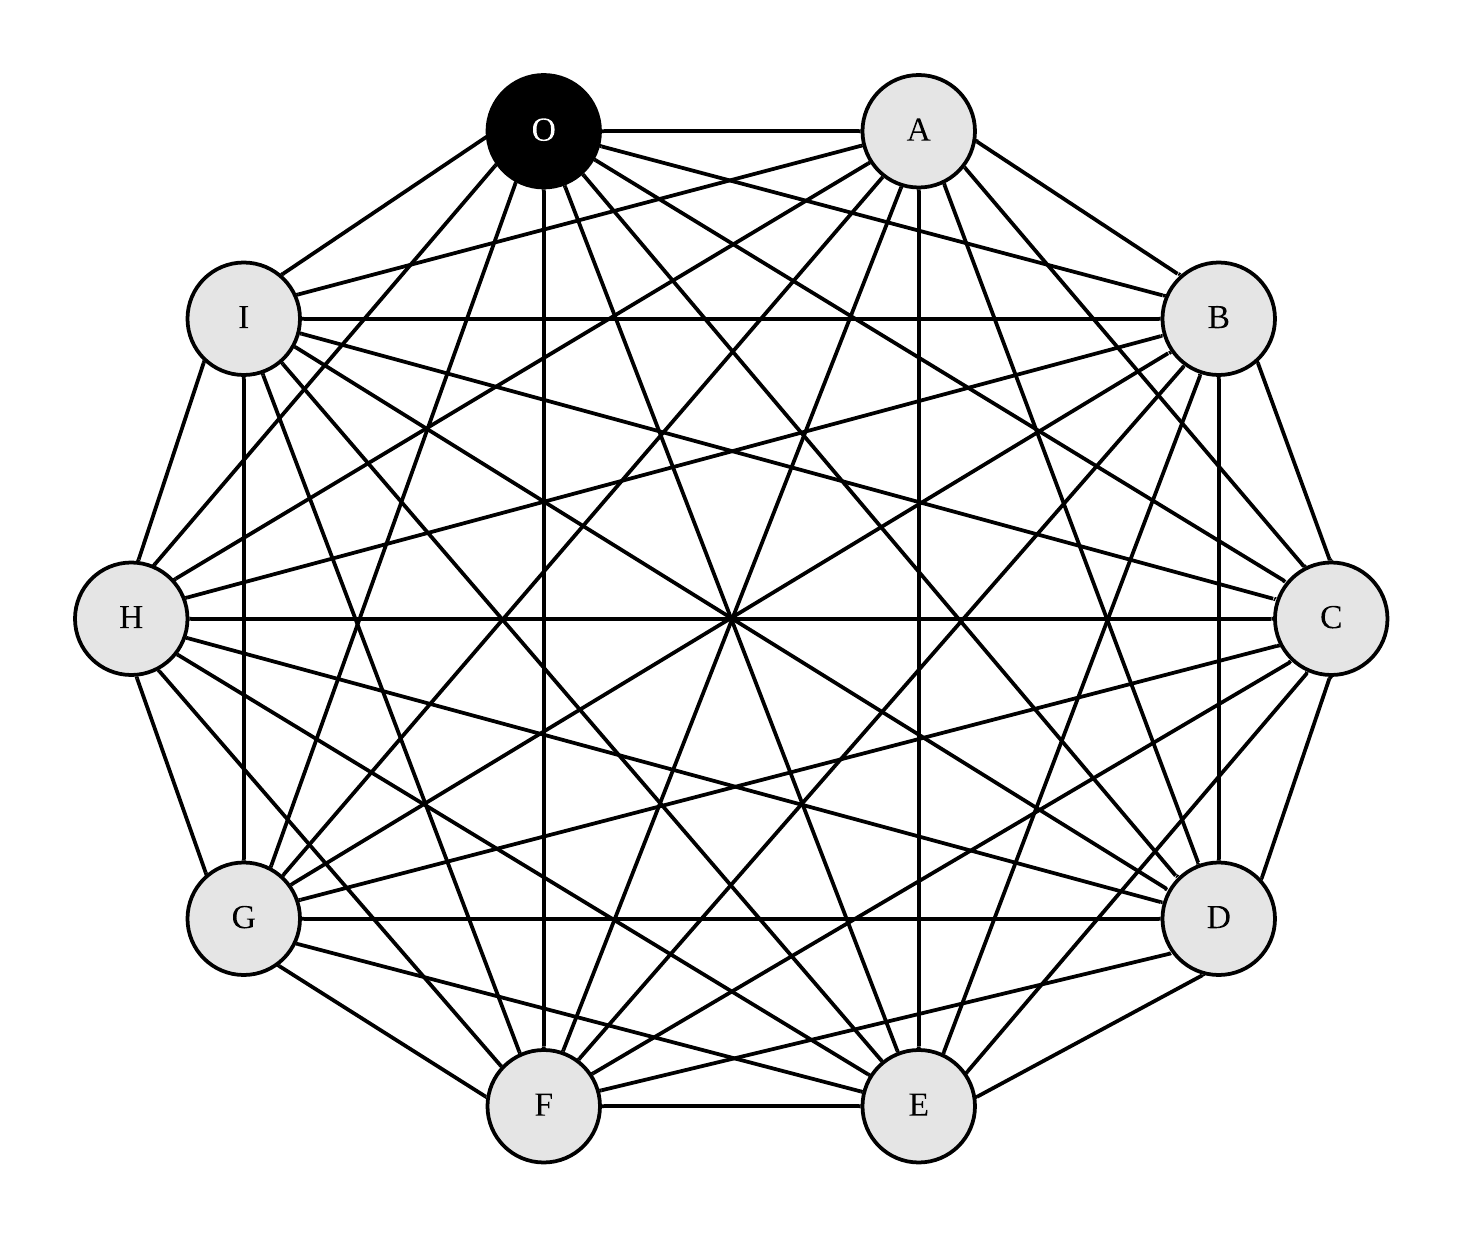
\includegraphics{TSP/images/CoffeeGraph.png}
    \caption{Introduction problem graph}
    \label{fig:my_label}
\end{figure}
\paragraph{Integer Linear Programming(ILP)} is a technique to accomplish the optimal result, (for example, most expensive or least cost) in a mathematical model whose necessities are defined  by linear relations. ILP defines decisions as variables and conditions by linear inequalities.\\
Let $(i,j)$ be any pair of cities in $\mathcal{N}$ such that $x_{ij}$ is defined as the decision variable and $c_{ij}$ is defined as the cost to travel between$\forall (i,j) \in \mathcal{N}$. Such that:\\
\begin{equation*}
    x_{ij} =    
    \begin{cases}
    1, & \text{if person travels immediately from $i$ to $j$} \\
    0, & \text{otherwise}    
    \end{cases}
\end{equation*}
The objective function is to minimise the total distance travelled which is defined as following:
\begin{equation*}
    \sum\sum_{(i,j)}c_{ij}x_{ij}
\end{equation*}
Given the following constraints
\begin{equation*}
    \sum_{j=1}^{n}x_{ij}\textnormal{  }\forall i
\end{equation*}
\begin{equation*}
    \sum_{i=1)}^{n}x_{ij}\textnormal{  }\forall j
\end{equation*}
The above constraints however are not enough as they do not eliminate sub-tours. A sub-tour is  a round tour that returns back to where you start, but does not visit all the cities. \\
Sub-tour elimination constraints:\\
\begin{equation*}
    x_{jj}=0
\end{equation*}
\begin{equation*}
    x_{ij} + x_{ji} <= 1
\end{equation*}

\section{Solution}
The Travelling Salesman problem is one that is classified as an NP-hard problem. NP stands for non-deterministic polynomial time. Thus these problems are problems which require polynomial time to be solved. Lets explore the viable options to find a solution to the problem.
\section*{Brute Force}
The first and most obvious algorithm  that comes to mind when looking at the problem is brute force. This algorithm simply calculates the length of every Hamiltonian cycle and chooses a solution with minimal length. Obviously this algorithm will have the optimal solution as outcome as it calculates every possible solution and keeps track of the minimum value. Lets look at Example 2 with a Brute force approach. Lets start of by listing all the possible Hamiltonian paths in the graph.
\begin{table}[H]
    \centering
    \begin{tabular}{|c|c|}
    \hline
    ~     & Path\\ 
    \hline
    \textbf{1}  & $O \to A \to B \to C \to O$         \\
    \textbf{2}  & $O \to A \to C \to B \to O$         \\
    \textbf{3}  & $O \to B \to A \to C \to O$         \\
    \textbf{4}  & $O \to B \to C \to A \to O$         \\
    \textbf{5}  & $O \to C \to A \to B \to O$         \\
    \textbf{6}  & $O \to C \to B \to A \to O$         \\
    \hline
    \end{tabular}
    \caption{Possible paths for Example 2}
    \label{tab:PathsExample1}
\end{table}

From Table \ref{tab:PathsExample1} we can see that there are 6 possible paths that Mark could take to complete his pub crawl. However, since  Mark's problem is one that is classified as a Symmetric TSP we know that the cost $c_{\overline{ab}} \in \mathcal{C}$ to travel between two cities $(a,b) \in \mathcal{N}$ is the same both ways: $c_{\overline{ab}}=c_{\overline{ba}}$. Thus from this we can infer that cost to take Path 1: $O \to A \to B \to C \to O$ would be the same as the cost for Path 6: $O \to C \to B \to A \to O$. This would also be true for Path 2/4 and Path 3/5. Thus halving the total number of paths from $(n-1)!$ to $\frac{(n-1)!}{2}.$\\
Thus now we can rule out Path 4/5/6 and calculate the cost of Path 1/2/3. Table \ref{tab:pubCrawlTotalCosts}
\begin{table}[H]
    \centering
    \begin{tabular}{|c|c|cc|}
    \hline
    ~     & Path& & Total cost\\ 
    \hline
    \textbf{1}&$O\to A\to B\to C\to O$&$294+557+448+394$&$=\textbf{1693}$  \\
    \textbf{2}&$O\to A\to C\to B\to O$&$294+656+448+307$&$=1705$  \\
    \textbf{3}&$O\to B\to A\to C\to O$&$307+557+656+394$&$=1914$  \\
    \hline
    \end{tabular}
    \caption{Total Costs for Example 1}
    \label{tab:pubCrawlTotalCosts}
\end{table}
From Table \ref{tab:pubCrawlTotalCosts} we can see that Path 1 has the least cost. This means that the best order in which Mark should go on his Pub Crawl is \textbf{Home $\to$ Lenehans Public House $\to$ Biddy Early's $\to$ O Riadas}. This trip would cost him 1693.\\
Let us now explore Example 1 with a similar Brute Force approach. Listing all the possible paths gives us the following paths:
\begin{table}[H]
    \centering
    \begin{tabular}{|c|c|c|c|}
    \hline
    ~     & Path&~&Path\\ 
    \hline
    \textbf{1}  & $O \to A \to B \to C \to D \to O$  &
    \textbf{13} & $O \to D \to C \to B \to A \to O$  \\
    \textbf{2}  & $O \to A \to B \to D \to C \to O$   &
    \textbf{13} & $O \to D \to C \to A \to B \to O$  \\

    \textbf{3}  & $O \to A \to C \to B \to D \to O$   &
    \textbf{15} & $O \to D \to B \to C \to A \to O$  \\

    \textbf{4}  & $O \to A \to C \to D \to B \to O$   &
    \textbf{16} & $O \to D \to B \to A \to C \to O$  \\

    \textbf{5}  & $O \to A \to D \to B \to C \to O$   &
    \textbf{17} & $O \to D \to A \to C \to B \to O$  \\

    \textbf{6}  & $O \to A \to D \to C \to B \to O$   &
    \textbf{18} & $O \to D \to A \to B \to C \to O$  \\

    \textbf{7}  & $O \to B \to A \to C \to D \to O$   &
    \textbf{19} & $O \to C \to D \to B \to A \to O$  \\

    \textbf{8}  & $O \to B \to A \to D \to C \to O$   &
    \textbf{20} & $O \to C \to D \to A \to B \to O$  \\

    \textbf{9}  & $O \to B \to C \to A \to D \to O$   &
    \textbf{21} & $O \to C \to B \to D \to A \to O$  \\

    \textbf{10} & $O \to B \to C \to D \to A \to O$   &
    \textbf{22} & $O \to C \to B \to A \to D \to O$  \\

    \textbf{11} & $O \to B \to D \to A \to C \to O$   &
    \textbf{23} & $O \to C \to A \to D \to B \to O$  \\

    \textbf{12} & $O \to B \to D \to C \to A \to O$  &
    \textbf{24} & $O \to C \to A \to B \to D \to O$  \\

    \hline
    \end{tabular}
    \caption{Possible paths for Example 2}
    \label{tab:PathsExample2}
\end{table}
Looking at Table \ref{tab:PathsExample2} we can tell that there are in total 24 paths. Additionally we can't discard any of the paths because this is an aTSP. Let us now calculate the cost(distance) of each path with the help of Table \ref{tab:suchirCostMatrix}.
\begin{table}[H]
    \centering
    \begin{tabular}{|c|c|c|c|}
    \hline
    Path No. & Total cost & Path no. & Total cost\\ 
    \hline
    \textbf{1} & 170+124+195+167+204=\textbf{860} & \textbf{13} & 199+179+182+106+147=\textbf{813}\\
    \textbf{2} & 170+124+ 81+ 70+276=\textbf{721} & \textbf{14} & 199+179+302+124+137=\textbf{941}\\
    \textbf{3} & 170+304+182+ 81+204=\textbf{941} & \textbf{15} & 199+70+195+302+147=\textbf{913}\\
    \textbf{4} & 170+304+167+ 70+137=\textbf{848} & \textbf{16} & 199+70+106+304+276=\textbf{955}\\
    \textbf{5} & 170+143+ 70+195+276=\textbf{854} & \textbf{17} & 199+134+304+182+137=\textbf{956}\\
    \textbf{6} & 170+143+179+182+137=\textbf{811} & \textbf{18} & 199+134+124+195+276=\textbf{928}\\
    \textbf{7} & 120+106+304+167+204=\textbf{901} & \textbf{19} & 199+167+70+106+147=\textbf{773}\\
    \textbf{8} & 120+106+143+179+276=\textbf{824} & \textbf{20} & 199+167+134+124+137=\textbf{845}\\
    \textbf{9} & 120+195+302+143+204=\textbf{964} & \textbf{21} & 199+182+81+134+147=\textbf{827}\\
    \textbf{10}& 120+195+107+134+147=\textbf{703} & \textbf{22} & 199+182+106+143+204=\textbf{918}\\
    \textbf{11}& 120+ 81+134+304+276=\textbf{915} & \textbf{23} & 199+302+143+70+137=\textbf{935}\\
    \textbf{12}& 120+ 81+179+302+147=\textbf{829} & \textbf{24} & 199+302+124+81+204=\textbf{994}\\
    \hline
    \end{tabular}
    \caption{Total Costs for Example 1}
    \label{tab:suchirTotalCosts}
\end{table}
From Table \ref{tab:suchirTotalCosts} we can see that Path 10 has the least cost. This means that the best order in which Suchir should go on his trip is \textbf{Home $\to$ Pharmacy $\to$ Bookstore $\to$ Restaurant $\to$ Supermarket $\to$ Home}. This trip would cost him 703.\\
Having a symmetric TSP helps a lot as it halves the total number of paths that need to be computed. However, in practical implementation we rarely get TSPs that are Symmetric and thus even though brute force always gives an optimal solution, for large n values the amount of operations that need to be done becomes incredibly high, even for a computer. Thus the number of paths that need to computed and compared increases exponentially. The table below shows how the number of paths increases with the number of nodes.
\begin{table}[H]
    \centering
    \begin{tabular}{|c|cccccccc|}
    \hline
    No. of nodes      &\textbf{2}&\textbf{3}&\textbf{4}&\textbf{5}&\textbf{10}&\textbf{20}&\textbf{50}&\textbf{100}\\
    \hline
    \textbf{sTSP}  & 1 & 1& 3 & 12 & 181440 & $6.082255\times10^{16}$ & $3.04140932\times10^{62}$ & $4.666311\times10^{155}$\\
    \textbf{aTSP}  & 1 &2& 6 & 24 & 362880 & $1.216451\times10^{17}$ & $6.08281864\times10^{62}$ &$9.332622\times10^{155}$\\
    \hline
    \end{tabular}
    \caption{Possible no. of paths for varying amount of nodes.}
    \label{tab:BruteForcePathsNumbers}
\end{table}
Looking at Table \ref{tab:BruteForcePathsNumbers} we can tell that the Brute Force approach become impractical at just 20 nodes to do by hand. As this would mean that the cost for every node has to be calculated and the value of the minimum has to be stores. Thus it makes it impossible for us to solve the introductory problem without the use of a computer. The graph below shows the relation between the number of nodes and number of possible paths. 
\begin{figure}[H]
    \centering
        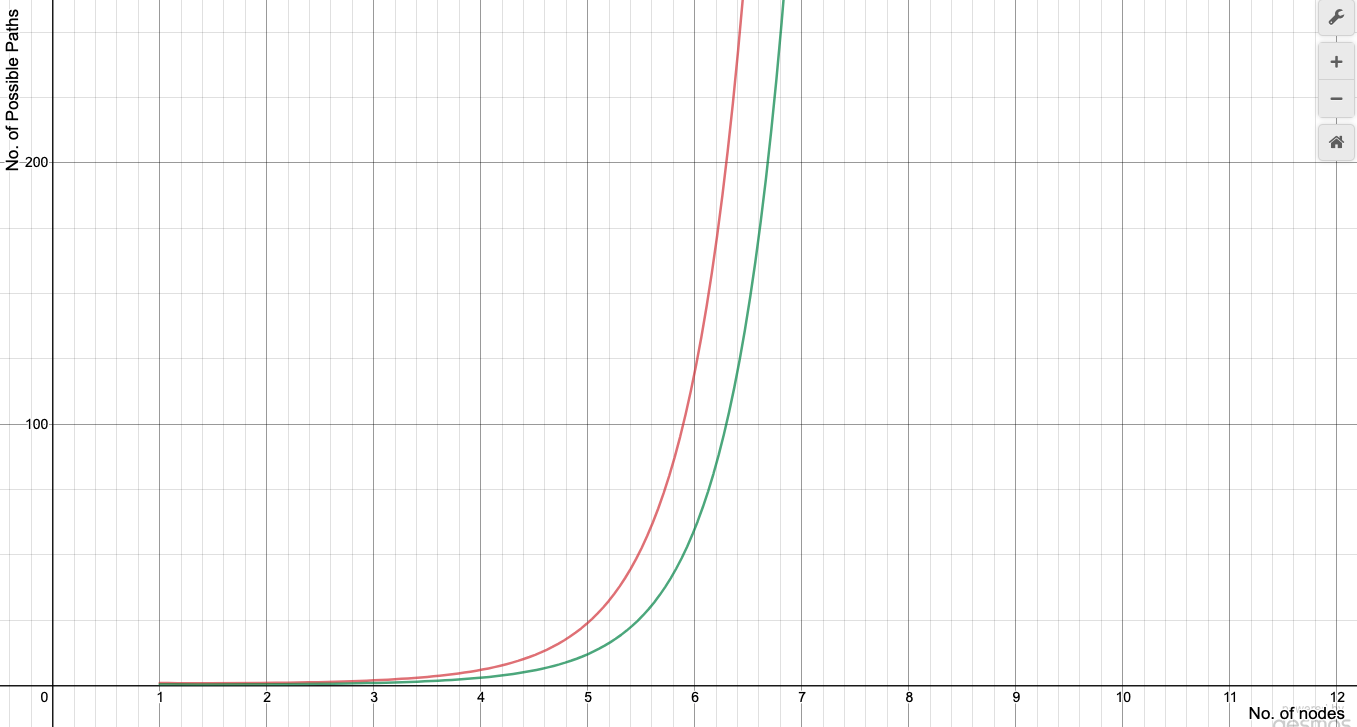
\includegraphics[width=150mm,scale=0.5]{TSP/images/graphNodesAndPaths.png}
        \caption{Nodes and Possible Paths}
        \label{fig:nodesAndPaths}
\end{figure}


This puts TSPs in a class of problems known as NP-hard. This means that TSP is classified as NP-hard because it has no “quick” solution and the complexity of calculating the best route will increase when you add more destinations to the problem. As we can see in Table \ref{tab:BruteForcePathsNumbers} for 10 nodes there are already more than 300,000 possibilities and for 20 more than 60 quadrillion possibilities this makes it difficult to solve the problem even for the fastest computers.\\
\section*{Nearest Neighbour Algorithm}
Another approach that could be taken to find a solution could be to visit the next minimum path. This is known as the Nearest Neighbour Algorithm.
Lets explore Example 2 using the nearest neighbour algorithm. The table below illustrates the possible paths Mark can take from the starting point and the cost for those paths:
\begin{table}[H]
    \centering
    \begin{tabular}{|c|c|}
    \hline
    Path & Cost\\ 
    \hline
    $O\to A$ & $294$  \\
    $O\to B$ & $307$  \\
    $O\to C$ & $394$  \\
    \end{tabular}
    \caption{}
    \label{tab:path1Mark}
\end{table}
Since $O\to A$ has the least cost Nearest Neighbour algorithm says to follow this path. This leaves us with the nodes B and C.
\begin{table}[H]
    \centering
    \begin{tabular}{|c|c|}
    \hline
    Path & Cost\\ 
    \hline
    $A\to B$ & $557$  \\
    $A\to C$ & $656$  \\
    \end{tabular}
    \caption{}

    \label{tab:path2Mark}
\end{table}
As per the above table we should go to B next as that is the nearest node. That leaves us with C and then returning back to the origin. This gives us the path $O\to A \to B \to C \to O$ which is the correct path, however, does that mean the nearest neighbour algorithm always gives the correct path? \\
Let us now explore the Example 1 using Nearest Neighbour Algorithm.
\begin{table}[H]
    \centering
    \begin{tabular}{|c|c|}
    \hline
    Path & Cost\\ 
    \hline
    $O\to A$ & $170$  \\
    $O\to B$ & $120$  \\
    $O\to C$ & $283$  \\
    $O\to D$ & $199$  \\
    \end{tabular}
    \caption{}
    \label{tab:path1Suchir}
\end{table}
From Table \ref{tab:path1Suchir} we can see that the shortest possible path is $O\to B$ which costs $120$. This leaves us with the following possibilities:
\begin{table}[H]
    \centering
    \begin{tabular}{|c|c|}
    \hline
    Path & Cost\\ 
    \hline
    $B\to A$ & $106$  \\
    $B\to C$ & $195$  \\
    $B\to D$ & $81$  \\
    \end{tabular}
    \caption{}
    \label{tab:path1Suchir}
\end{table}
Since $B\to D$ has the least cost of $81$ we consider path $B\to D$. Leaving us with:
\begin{table}[H]
    \centering
    \begin{tabular}{|c|c|}
    \hline
    Path & Cost\\ 
    \hline
    $D\to A$ & $134$  \\
    $D\to C$ & $179$  \\
    \end{tabular}
    \caption{}
    \label{tab:path1Suchir}
\end{table}
$D\to A$ is the least here. This gives us the path: $O\to B \to D \to A \to C \to O$. This path is Path no. 11. As you can see this is a different answer from the Brute force approach.
\begin{table}[h]
    \centering
    \begin{tabular}{|c|c|cc|}
    \hline
    TSP & No. of Nodes & Real Solution/Brute Force & Nearest Neighbour Solution \\ \hline
    Example 1      & \textbf{5}   & 703  & 915\\
    Example 2      & \textbf{4}   & 1693 & 1693\\
    \end{tabular}
    \caption{Total cost using Brute Force and NN Algorithm}
    \label{tab:eg1CostMatrix}
\end{table}
As you can see from the above table the nearest neighbour algorithm does not always give the most optimal solution. It helps us to get an upper bound of the solution. Thus nearest neighbour is classified as an approximation method to solve the TSP.\\
Finding a solution to the introduction problem without the help of a computer would take a lot of time. As we can see for a 5 node aTSP we has 24 possible paths. For a 10 node sTSP we would have 181440 possible paths making it impossible to do by hand. Thus for this purpose we would be making use of a computer to solve the introductory problem in the next section.
\section{Computational Complexity}
As mentioned before the TSP is classified as an NP hard problem one which requires polynomial time to be solved. To explore the time taken to solve TSP problems for varying nodes and to calculate the solution to the introductory problem, I authored computer algorithm to calculate the time taken for different number of nodes using NN-Algorithm and Brute force approach. In addition to the 4 nodes from Example 2, 5 nodes from Example 1 and 10 nodes from the introduction problem. I will be making use of well known sTSP problems: att48-48 capitals of the US\cite{att48}, and bier127-127 Biergaerten in Augsburg\cite{bier127}. The solution attained using the computer and the time taken to execute each test is displayed below:
\begin{table}[H]
\begin{tabular}{|c|c|c|c|c|c|c|c|c|c|c|c|}
\hline
\multicolumn{2}{|c|}{-}                                                                  & \multicolumn{5}{c|}{Execution time/s}  & \multicolumn{5}{c|}{Computer solution} \\ \hline
\multicolumn{2}{|c|}{No. of Nodes}                                                       & 4     & 5     & 10     & 48    & 127   & 4     & 5    & 10   & 48     & 127     \\ \hline
\multirow{2}{*}{Algorithm} & \begin{tabular}[c]{@{}c@{}}Brute\\  Force\end{tabular}      & 0.012 & 0.019 & 16.823 & NA    & NA    & 1693  & 703  & 740  & NA     & NA      \\ \cline{2-12} 
                           & \begin{tabular}[c]{@{}c@{}}Nearest\\  Neighbour\end{tabular} & 0.074 & 0.085 & 0.099  & 0.122 & 0.209 & 1693  & 915  & 878  & 40526  & 159678  \\ \hline
\end{tabular}
\end{table}
WE can see from the table above how even for a computer the time taken to calculate the solution for an sTSP with 10 nodes increases from 0.019 seconds for 5 to 16.8 second 10. However it has to be noted that this value may vary from computer to computer. However, since this experiment was done on the same device it keeps the computational capability of the laptop constant. Additionally, the computer was unable to calculate the number 48 and 127 nodes as it would take nearly 20 years to compute a solution using the computer used just for the 48 nodes. We can see from solution provided that the least cost for the introduction problem was 740 and the path was: 
\begin{center}
     O$\to$C$\to$A$\to$B$\to$D$\to$E$\to$F$\to$G$\to$I$\to$H$\to$O
\end{center}
we can see that smaller problems up to around 20 nodes are solvable(optimal solution) with the help of a computer easily because of their calculation capability however solving a TSP without a computer becomes impractical at just 5 nodes. Thus for larger problems we need to make use of algorithms that may not give the best solution however give an estimation for the real solution. These algorithms are make use of heuristic approaches to estimating the solution to TSP. When finding a solution for the TSP there is always a trade off between accuracy and time.

\section{Conclusion}
The travelling salesman problem plays a significant role in industries that are of huge importance to our daily lives. Such as X-Ray crystallography, Drilling of printed circuit boards, Printing press scheduling and even school bus routing. The wide pertinence of the TSP model,  and the trouble of finding an optimal solution makes the TSP a fascinating and significant issue in applied science. The TSP is one of a handful of  problems that mathematicians turn to again and again to test the limits of computation.\\
Also, TSP has now allowed us to solve our introduction problem relating as we now know the shortest route the coffee delivery boy can take helping him optimise his way around the school.\\
\begin{center}
     O$\to$C$\to$A$\to$B$\to$D$\to$E$\to$F$\to$G$\to$I$\to$H$\to$O\\
     740
\end{center}
As our knowledge of algorithms progresses and technology advances we would be able to solve large TSPs helping provide real world solutions in various fields.
\newpage

\printbibliography

\end{document}


